% !TEX encoding = UTF-8 Unicode 
\begin{filecontents*}{\jobname.xmpdata}
\Title{Opinnäytetyö}
\Author{Noora Angelva}
\end{filecontents*}

% Yllä on määritelty pdf/a-muotoon vaadittu metadata minimaalisella tavalla
%Tämän LaTeX-pohjan laadintaan ovat osallistuneet Mika Hirvensalo, Teemu Pirttimäki, Petriina Paturi ja Vesa Halava

\documentclass[a4paper,12pt,oneside]{article} % yksipuolinen
\usepackage[finnish]{babel}            				% suomenkielinen tavutus ja sanasto
\usepackage[T1]{fontenc}               				% valitaan ääkkösfonttikoodaus
\usepackage[utf8]{inputenc}        						% skandit utf-8 koodauksella
\usepackage{amsthm}														% theorem- yms. ympäristöt
\usepackage{amsmath}													% AMS-matematiikkatoimintoja
\usepackage{graphicx}           							% kuvat
%\usepackage[dvips]{graphicx}           			% ps-kuvat
\usepackage{graphicx,wrapfig,lipsum}

% Seuraavat rivit määrittävät LaTeXin oletusfontin Computer Modern sijasta käytettäväksi New TX-fontin. Poista 
% rivien ensimmäinen % jos tahdot käyttää New TX-fonttia.
%%%%%%%%%%%%%%%%%%%%%%%%%%%%%%%%%%%%%%%%%%%%%%%%
%\usepackage{newtxtext}       
%\usepackage{newtxmath}
%%%%%%%%%%%%%%%%%%%%%%%%%%%%%%%%%%%%%%%%%%%%%%%%
\usepackage[tagpdf]{axessibility} %Saavutettavuuspaketti, kaavoista tulee lukuohjelmalla luettavampia
%HUOM: LaTeXin erillinen accessibility-paketti ei toimi amsthm-paketin kanssa.
%%%%%%%%%%%%%%%%%%%%%%%%%%%%%%%%%%%%%%%%%%%%%%%%
% Seuraavat rivit määrittävät saavutettavuuden kannalta riittävän pdf/a-muodon UTUGradu-järjestelmään.
% Gradua voi olla mukavampi työstää ilman näitä, ne voi ottaa käyttöön vasta 

%%%%%%%%%%%%%%%%%%%%%%%%%%%%%%%%%%%%%%%%%%%%%%%%

\usepackage[a-3b]{pdfx}  											% Lähtökohtana pdf/a-3b
\usepackage[pdfa]{hyperref}										% pdf/a-muotoa varten



%%%%%%%%%%%%%%%%%%%%%%%%%%%%%%%%%%%%%%%%%%%%%%%%
% Testauksen vuoksi pseudolatinaa tuottava
% paketti. Et tarvitse tätä omassa työssäsi.
\usepackage{lipsum}  
%%%%%%%%%%%%%%%%%%%%%%%%%%%%%%%%%%%%%%%%%%%%%%%%

% Helvetica-fontti on LaTeXin helposti käytettävissä olevista fonteista lähinnä yliopiston suositusfonttia
% Poista seuraavien rivien ensimmäinen % ja poista ylläolevat rivit jos tahdot käyttää tätä fonttia.

%%%%%%%%%%%%%%%%%%%%%%%%%%%%%%%%%%%%%%%%%%%%%%%%
%\renewcommand{\familydefault}{\sfdefault}
%\usepackage[scaled=1]{Arial}
%\usepackage[Arial]{sfmath}
%\everymath={\sf}

\renewcommand{\rmdefault}{phv} % Arial
\renewcommand{\sfdefault}{phv} % Arial
%%%%%%%%%%%%%%%%%%%%%%%%%%%%%%%%%%%%%%%%%%%%%%%%

% A4 mitat ovat 210x297 (mm), ylämarginaali 30 mm, vasen marginaali 30 mm

% Lapin AMK
% 40 mm vasen reuna lapinamk
% 20 mm ylä- ja oikreuna lapinamk
% 210 - 40 - 20 = 150 leveys
% 297 - 20 -20 = 257 korkeus
%%%%%%%%%%%%%%%%%%%%%%%%%%%%%%%%%%%%%%%%%%%%%%%%
\usepackage{geometry}
\geometry{
 a4paper,
 total={150mm,257mm},
 left=40mm,
 top=20mm,
 }



%Suomenkieliset ympäristöt: 

\theoremstyle{plain}
\newtheorem{theorem}{Lause}
\newtheorem{lemma}{Lemma}
\newtheorem{corollary}{Seuraus}
%
\theoremstyle{definition}
\newtheorem{definition}{M\"a\"aritelm\"a}
\newtheorem{example}{Esimerkki}
%
\theoremstyle{remark}
\newtheorem{remark}{Huomautus}

%Määrittele tässä aika, työn, kirjoittajan ja ohjaajien tiedot

\newcommand{\tekija}{{Noora Angelva}} %tekijän nimi
\newcommand{\Ohjaajat}{{Maisa Mielikäinen ja Tuija x}} %tekijän nimi
\newcommand{\Toimeksiantaja}{{Yhtiö X}} %tekijän nimi
\newcommand{\titteli}{{ }} %voi jättää tyhjäksi
\newcommand{\otsikko}{{Headline}}   %Gradun otsikko
\newcommand{\tutkielma}{{Thesis}}   %Pro Gardu tai LuK. Huom kirjoitusasu, välilyönti lopussa graduille
\newcommand{\aika}{{2021}}   %vuosi
\newcommand{\tutkintonimike}{{Engineer of Information and Communication Technology}} %tai Tilastotiede
\newcommand{\tutkintonimikeFin}{{Tieto- ja viestintätekniikan insinööri}}
\newcommand{\Koulutus}{{Engineer (Bachelor)}}
\newcommand{\KoulutusFin}{{Insinööri (AMK)}}
\newcommand{\opinnaytetyo}{{Opinäytetyö}} %Opinnatetyo (Prof./Dos./FT) ja nimi 
\newcommand{\koulutus}{{Koulutus}} %Koulutus


\begin{document}
\pagenumbering{arabic} %Saavuttavuuden takija alussa sivunurot roomalaisittain, tutkielman alusta arabialaisittain.
\pagestyle{empty}  %ei sivunumeroa sivun alareunaan

\begin{center}

\includegraphics[width=6cm]{UAS_Logo}
\end{center}

% korjaa fontti koko ja korkeus
\vspace{3.0cm}
\begin{center}\LARGE
\otsikko 
\end{center}

% korjaa korkeus
\vspace{9cm}
\begin{center}
\tekija
\end{center}

\vspace{0.5cm}
\begin{center}
\opinnaytetyo 
\\ \koulutus
\\ \tutkintonimike
\\ \end{center}

%korjaa koko ja korkeus
\vspace{0.5cm}
\begin{center}\LARGE
\aika
\end{center}

% TIIVISTELMÄ (EN) %

\newpage\null
\pagestyle{empty}  %ei sivunumeroa sivun alareunaan
\vspace{1.27cm}

% YLATUNNISTE
% Tahan jaaty korjaa, vasen reuna (40mm)
\noindent\begin{minipage}{0.4\textwidth}
\noindent
\includegraphics[width=4.83cm]{ylatunnisteLogo}
\end{minipage}
\begin{minipage}{0.6\textwidth}\raggedleft
Opinnäytetyön tiivistelmä\\
\end{minipage}
%\vspace{0.5cm}
\noindent \Koulutus \\
\tutkintonimike \\
\rule{\textwidth}{.2mm}\\

% YLATUNNISTE END
%
% Tahan jaaty korjaa, vasen reuna (40mm)
%

\vspace{1mm}\noindent \textbf{Author} \	\tekija\\
\vspace{1mm}\noindent \textbf{Year} \	\aika \\
\vspace{1mm}\noindent \textbf{Supervisor(s)}	\ \Ohjaajat \\
\vspace{1mm}\noindent \textbf{Commissioned by}	\ \Toimeksiantaja \\
\vspace{1mm}\noindent \textbf{Subject of thesis} \	\opinnaytetyo \\
\vspace{1mm}\noindent \textbf{Number of pages} \	XX + X \\
\rule{\textwidth}{.2mm}\\

%TIIVISTELMÄ ->

\vspace{4mm}\noindent Kirjoita tähän tiivistelmä. Laita $\backslash${noindent}-komento kappaleen
alkuun, niin \LaTeX\, ei sisennä ensimmäistä riviä.

\vspace{4mm}\noindent Komento $\backslash$vspace taasen jättää sopivan välin kappaleiden väliin - 4mm näyttää aika hyvältä.

\vspace{4mm}\noindent Kirjoita tiivistelmä napakasti ja kaikenlaista toistoa välttäen.

\vspace{4mm}\noindent Keywords: tiivistelmäsivu, Pro gradu -tutkielma, \LaTeX-ladontajärjestelmä.


% TIIVISTELMÄ (FIN) %

\newpage\null
\pagestyle{empty}  %ei sivunumeroa sivun alareunaan
\vspace{1.27cm}

% YLATUNNISTE
\noindent\begin{minipage}{0.4\textwidth}
\noindent
\includegraphics[width=4.83cm]{ylatunnisteLogo}
\end{minipage}
\begin{minipage}{0.6\textwidth}\raggedleft
Opinnäytetyön tiivistelmä\\
\end{minipage}\
%\vspace{0.5cm}
\noindent\KoulutusFin \\
\tutkintonimikeFin \\
\rule{\textwidth}{.2mm}\\
% YLATUNNISTE END

\vspace{1mm}\noindent \textbf{Tekijä} \	\tekija\\
\vspace{1mm}\noindent \textbf{Vuosi} \	\aika \\
\vspace{1mm}\noindent \textbf{Ohjaaja(t)}	\ \Ohjaajat \\
\vspace{1mm}\noindent \textbf{Toimeksiantaja}	\ \Toimeksiantaja \\
\vspace{1mm}\noindent \textbf{Työn nimi} \	\opinnaytetyo \\
\vspace{1mm}\noindent \textbf{Sivu- ja liitesivumäärä} \	XX + X \\
\noindent\rule{\textwidth}{.2mm}\\


% TIIVISTELMä ->

\vspace{4mm}\noindent Kirjoita tähän tiivistelmä. Laita $\backslash${noindent}-komento kappaleen
alkuun, niin \LaTeX\, ei sisennä ensimmäistä riviä.

\vspace{4mm}\noindent Komento $\backslash$vspace taasen jättää sopivan välin kappaleiden väliin - 4mm näyttää aika hyvältä.

\vspace{4mm}\noindent Kirjoita tiivistelmä napakasti ja kaikenlaista toistoa välttäen.

\vspace{4mm}\noindent Asiasanat: tiivistelmäsivu, Pro gradu -tutkielma, \LaTeX-ladontajärjestelmä.


% SISALLYSLUETTELO %

\newpage\null
\tableofcontents
%Aja laTeX-käännös uudelleen saadaksesi ajantasaisen sisällysluettelon
%\cleardoublepage


% TEKSTI OSUUS %

\newpage\null
\pagestyle{plain} 

\section{Alkusanat}

Tässä luvussa esitetään niin kutsuttu Newtonin-Leibnizin kaava \cite{NewtLeib}.

\begin{theorem} Oletetaan että välillä $[a,b]$ on $F'(x)=f(x)$ ja että $f$ on jatkuva.\footnote{Jatkuvuus on oleellinen seikka tässä yhteydessä.} Tällöin
\[
\int_a^bf(x)\,dx=F(b)-F(a).
\]
\end{theorem}

\subsection{Analyyttistä lukuteoriaa}

Seuraavaksi esitellään niin sanottu {\em Riemannin hypoteesi}, jonka mukaan ns. $\zeta$-funktion epätriviaalit nollakohdat sijaitsevat suoralla $\operatorname{Re}z=\frac12$.
\begin{definition} Riemannin $\zeta$-funktio määritellään sarjaesityksen \cite{Riemann}
\[
\zeta(z)=\sum_{n=1}^{\infty}\frac{1}{n^z}
\]
avulla, kun $\operatorname{Re}z>1$.
\end{definition}

\subsubsection{Matriisilaskentaa}

Nyt tarkastellaan matriisin
\[
A=\left(\begin{array}{rrr} -1 & -2 & -5\\ 3& 4& 5\\ -3 & 2 & 1 \end{array}\right)
\]
ominaisarvoja.

\section{Käytetyt merkit ja lyhenteet}

UTUGradu-järjestelmän ja PDF\LaTeX :n pdf-formaattivaatimusten takia kannattaa käyttää muita kuin eps-muotoisia kuvia. Esimerkiksi pdf-muoto käy mainiosti vektorikuville, kunhan on samaa pdf/a-3b muotoa kuin tämän tiedoston tuottama pdf-tiedosto. Parhaiten toimivat jpg-muotoiset kuvat.



\subsection{Saavutettavuus kuvateksteissä}

Kaikkiin tutkielmassa esiintyviin kuviin tulee viitata tekstissä (ks.~\ref{kuvatus1}) Lisäksi kuvatekstin tulee olla kuvaileva, koska saavutettavuuteen liittyvät alt-tekstit eivät oikein toimi käytetyn \LaTeX :n axessibility-paketin kanssa. Jos kuvan perusteella tehdään päätelmä, tulee päätelmä kuvata tekstissä. 

\begin{figure}[ht]
\begin{center}
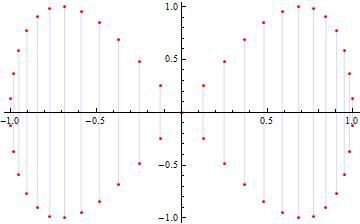
\includegraphics[width=.45\textwidth]{siivet.jpg}
\end{center}
\label{kuvatus1}
\caption{Geronon lemniskaatta välillä $[-1,1]$.}
\end{figure}

\section{Johdanto}

\lipsum[1-10]


%Kirjallisuusluettelon määrittelyssä {99} on levein kirjallisuusviitteen numero. Oikaise tarvittaessa.
 
\begin{thebibliography}{99}

\bibitem{NewtLeib} Newton ja Leibniz

\bibitem{Riemann} Riemann

\end{thebibliography}
\end{document}
